% #############################################################################
% This is Chapter 5
% !TEX root = ../main.tex
% #############################################################################
% Change the Name of the Chapter i the following line
\fancychapter{Experiments}
\cleardoublepage
% The following line allows to ref this chapter
\label{chap:evaluation}

This chapter presents the comprehensive evaluation of our open-vocabulary aerial image segmentation approach using the AerialD dataset and RSRefSeg architecture. We describe the model architecture, experimental setup, quantitative and qualitative results, and ablation studies.

% #############################################################################
\section{Model Architecture}

Our approach implements the RSRefSeg architecture, as illustrated in Figure \ref{fig:rsrefseg_architecture} from Chapter 3, which combines text and visual understanding for precise object segmentation in aerial imagery. We selected this architecture for its versatility in enabling both referring instance segmentation and semantic segmentation, allowing the model to segment both individual objects and broader semantic regions effectively. The architecture leverages two robust vision foundation models as backbones: SigLIP2 for vision-language encoding and SAM for mask generation, providing a solid foundation built on proven components with strong pre-trained capabilities.

We implemented this architecture from scratch in PyTorch, faithfully following the original RSRefSeg paper design and verified its effectiveness by replicating the reported results on the RRSIS-D dataset. The model employs LoRA (Low-Rank Adaptation) for efficient fine-tuning, enabling parameter-efficient training while maintaining the strong pre-trained representations from the foundation models. This approach allows us to adapt the powerful vision-language capabilities to the specific domain of aerial imagery while minimizing computational requirements during training.

% #############################################################################
\section{Experimental Setup}

Our training configuration uses a batch size of 4 with gradient accumulation steps of 2, resulting in an effective batch size of 8 samples. The model employs LoRA fine-tuning for parameter-efficient adaptation, targeting the query and value projection layers in both the SigLIP2 vision encoder and SAM vision encoder, and the query, key, value, and output projection layers in the text encoder. We use the google/siglip2-so400m-patch14-384 model for vision-language encoding and facebook/sam-vit-base for mask generation. Training uses AdamW optimizer with an initial learning rate of 1e-4, weight decay of 0.01, and polynomial learning rate decay with power factor 0.9. The pipeline leverages mixed-precision computation for efficiency and applies gradient clipping with maximum norm of 1.0 for stability. All images are resized to 384×384 pixels to match the SigLIP2 input requirements.

Our experimental design centers on training models using the AerialD dataset and evaluating performance through cross-dataset evaluation on three established aerial referring segmentation benchmarks: RefSegRS, RRSIS-D, and NWPU-Refer. This cross-evaluation approach validates the generalization capabilities of models trained on our dataset when applied to different aerial imagery domains, annotation styles, and expression patterns.

To understand the individual contributions of different expression types within AerialD, we train various model variants on different subsets of our dataset alongside the complete combined dataset. These variants include models trained exclusively on rule-based expressions, language variation expressions only, unique visual detail expressions only, and the full combined dataset incorporating all expression types. The comparative analysis of these variants, detailed in the ablation studies section, provides insights into how different enhancement strategies affect model performance and generalization across diverse referring expression patterns.


% #############################################################################
\section{Evaluation Results}

Our evaluation demonstrates that the model trained on AerialD generalizes effectively to other aerial referring segmentation datasets. The cross-dataset performance evaluation presented in Table \ref{tab:cross_dataset_results} shows that our approach maintains reasonable performance when applied to RefSegRS, RRSIS-D, and NWPU-Refer datasets, despite being trained exclusively on AerialD. This generalization capability indicates that the diversity and scale of expressions in our dataset enable the model to adapt to different annotation styles, object categories, and expression patterns found in other aerial imagery domains.

% Cross-dataset performance table
\begin{table}[H]
\centering
\caption{Cross-Dataset Performance Evaluation - Model Trained on Aerial-D Only (Historic-filtered results in \textcolor{blue}{blue})}
\label{tab:cross_dataset_results}
\begin{tabular}{@{}lcccccccc@{}}
\toprule
\textbf{Dataset} & \textbf{IoU@0.5} & \textbf{IoU@0.7} & \textbf{IoU@0.9} & \multicolumn{2}{c}{\textbf{mIoU}} & \multicolumn{2}{c}{\textbf{oIoU}} \\
\cmidrule(lr){5-6} \cmidrule(lr){7-8}
 & & & & \textbf{Orig.} & \textbf{Hist.} & \textbf{Orig.} & \textbf{Hist.} \\
\midrule
Aerial-D & -- & -- & -- & -- & \textcolor{blue}{--} & 50.3\% & \textcolor{blue}{--} \\
RRSIS-D & 32.87\% & 23.39\% & 10.34\% & 34.07\% & \textcolor{blue}{32.44\%} & 34.80\% & \textcolor{blue}{34.33\%} \\
NWPU-Refer & 25.68\% & 15.91\% & 4.02\% & 24.57\% & \textcolor{blue}{20.66\%} & 28.27\% & \textcolor{blue}{20.12\%} \\
RefSegRS & 15.55\% & 1.86\% & 0.00\% & 18.80\% & \textcolor{blue}{14.75\%} & 8.58\% & \textcolor{blue}{4.65\%} \\
\bottomrule
\end{tabular}
\end{table}

% Combined training performance table
\begin{table}[H]
\centering
\caption{Combined Training Performance Evaluation - Model Trained on All Dataset Train Sets (Historic-filtered results in \textcolor{blue}{blue})}
\label{tab:combined_training_results}
\begin{tabular}{@{}lcccccccc@{}}
\toprule
\textbf{Dataset} & \textbf{IoU@0.5} & \textbf{IoU@0.7} & \textbf{IoU@0.9} & \multicolumn{2}{c}{\textbf{mIoU}} & \multicolumn{2}{c}{\textbf{oIoU}} \\
\cmidrule(lr){5-6} \cmidrule(lr){7-8}
 & & & & \textbf{Orig.} & \textbf{Hist.} & \textbf{Orig.} & \textbf{Hist.} \\
\midrule
Aerial-D & -- & -- & -- & -- & \textcolor{blue}{--} & -- & \textcolor{blue}{--} \\
RRSIS-D & -- & -- & -- & -- & \textcolor{blue}{--} & -- & \textcolor{blue}{--} \\
NWPU-Refer & -- & -- & -- & -- & \textcolor{blue}{--} & -- & \textcolor{blue}{--} \\
RefSegRS & -- & -- & -- & -- & \textcolor{blue}{--} & -- & \textcolor{blue}{--} \\
Urban1960SatSeg & -- & -- & -- & -- & N/A & -- & N/A \\
\bottomrule
\end{tabular}
\end{table}

% Dataset comparison table
\begin{table}[H]
\centering
\caption{Comparison with Existing RRSIS Datasets}
\label{tab:dataset_comparison}
\resizebox{\textwidth}{!}{%
\begin{tabular}{@{}lccccccr@{}}
\toprule
\textbf{Dataset} & \textbf{Image Resolution} & \textbf{Images} & \textbf{Annotations} & \textbf{Single-object} & \textbf{Multi-object} & \textbf{Resolution} & \textbf{Annotation Generation} \\
\midrule
RefSegRS & 0.13m & 4420 & 4420 & \checkmark & $\times$ & 512 & Manual \\
RRSIS-D & 0.5m-30m & 17402 & 17402 & \checkmark & $\times$ & 800 & Semi-auto \\
NWPU-Refer & 0.12m-0.5m & 15003 & 49745 & \checkmark & \checkmark & 1024-2048 & Manual \\
\midrule
\textbf{AERIAL-D} & \textbf{0.3m-4.5m} & \textbf{43,514} & \textbf{1,545,994} & \textbf{\checkmark} & \textbf{\checkmark} & \textbf{480} & \textbf{Automated + LLM} \\
\bottomrule
\end{tabular}%
}
\end{table}

Our dataset comparison presented in Table \ref{tab:dataset_comparison} reveals that AerialD represents a significant advancement in aerial referring segmentation datasets. With over 1.5 million referring expressions, it surpasses the largest existing dataset by more than 30-fold. Notably, AerialD is the first dataset to achieve fully automated annotation generation without manual intervention, combining rule-based expression generation with LLM enhancement. The dataset supports both single-object and multi-object referring expressions, making it more comprehensive than previous datasets that focus primarily on single-object scenarios.

\begin{figure}[H]
\centering
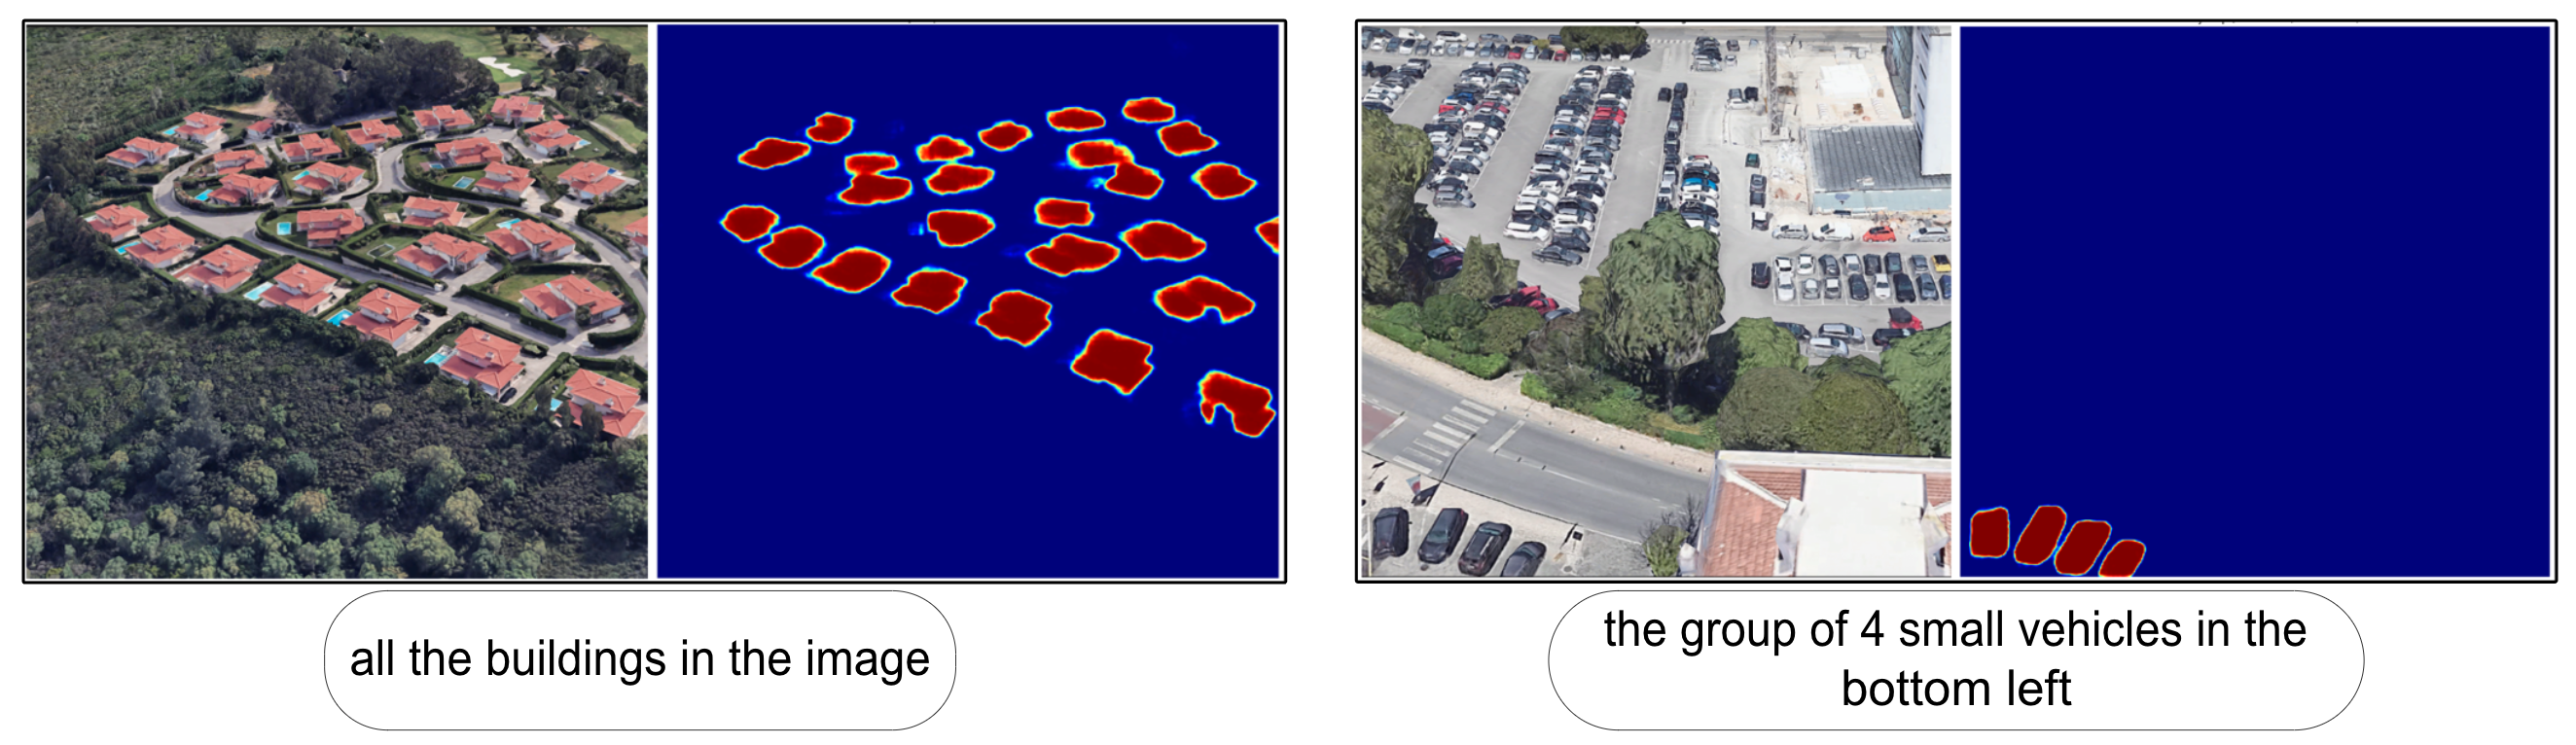
\includegraphics[width=\textwidth]{Images/qualitative.png}
\caption{Qualitative segmentation results from RSRefSeg model on Google Earth imagery.}
\label{fig:qualitative_examples}
\end{figure}

The qualitative results shown in Figure \ref{fig:qualitative_examples} demonstrate the model's generalization capabilities through successful segmentation of objects in Google Earth imagery, which differs from the training data sources. The figure displays probability heatmaps generated by the model, where higher probability regions (shown in red) indicate the model's confidence in object localization. The left example shows the model successfully identifying "all the buildings in the image" across a residential area with red-roofed houses, accurately capturing the spatial distribution of individual structures. The right example demonstrates precise localization of "the group of 4 small vehicles in the bottom left" within a complex parking area, showing the model's ability to distinguish specific vehicle groups from the surrounding context. These results indicate that the model can effectively transfer its learned representations to new imagery domains while maintaining precise object localization and segmentation quality.

% #############################################################################
\section{Ablation Studies}

To evaluate the individual contributions of different expression enhancement strategies, we conduct an ablation study comparing models trained on different subsets of the AerialD dataset. The primary motivation behind this analysis is to determine whether the LLM enhancement process positively impacts model performance and to quantify the benefits of each enhancement type. As detailed in Table \ref{tab:llm_enhancement_stats} from Chapter 4, our dataset contains approximately 506K rule-based expressions, 497K language variation expressions, and 519K unique visual detail expressions, totaling 1.52M expressions.

% Ablation expression types table
\begin{table}[H]
\centering
\caption{Ablation Study: Cross-Dataset Performance by Training Configuration}
\label{tab:ablation_expression_types}
\resizebox{\textwidth}{!}{%
\begin{tabular}{@{}lc|ccc|ccc|ccc|ccc@{}}
\toprule
\multirow{2}{*}{\textbf{Training Configuration}} & \multirow{2}{*}{\textbf{Samples}} & \multicolumn{3}{c|}{\textbf{Aerial-D}} & \multicolumn{3}{c|}{\textbf{RefSegRS}} & \multicolumn{3}{c|}{\textbf{RRSIS-D}} & \multicolumn{3}{c}{\textbf{NWPU-Refer}} \\
\cmidrule(lr){3-5} \cmidrule(lr){6-8} \cmidrule(lr){9-11} \cmidrule(lr){12-14}
 & & \textbf{Pass@0.7} & \textbf{mIoU} & \textbf{oIoU} & \textbf{Pass@0.7} & \textbf{mIoU} & \textbf{oIoU} & \textbf{Pass@0.7} & \textbf{mIoU} & \textbf{oIoU} & \textbf{Pass@0.7} & \textbf{mIoU} & \textbf{oIoU} \\
\midrule
Rule-based Only & 506K × 4 & -- & -- & -- & -- & -- & -- & -- & -- & -- & -- & -- & -- \\
Language Variations Only & 497K × 4 & -- & -- & -- & -- & -- & -- & -- & -- & -- & -- & -- & -- \\
Unique Expressions Only & 519K × 4 & -- & -- & -- & 2.55\% & 18.32\% & 8.37\% & 20.86\% & 31.78\% & 33.73\% & 15.91\% & 24.68\% & 29.22\% \\
Combined All & 1,522K × 2 & -- & -- & 50.3\% & 1.86\% & 18.80\% & 8.58\% & 23.39\% & 34.07\% & 34.80\% & 15.91\% & 24.57\% & 28.27\% \\
\bottomrule
\end{tabular}%
}
\end{table}

To ensure fair comparison across different training configurations, we carefully control the total number of training samples each model observes during training. Since the combined dataset contains approximately 1.52M expressions, we train the individual subset models for 3 epochs each, resulting in roughly 1.5M samples seen, which closely matches the number of unique samples in the full combined dataset trained for 1 epoch. This methodology prevents comparing "apples to oranges" by ensuring that performance differences arise from data quality and diversity rather than simply the quantity of training samples observed.

The ablation results demonstrate that the combined model, utilizing all expression types, achieves the best performance across all evaluation metrics on the AerialD validation set. This validates our hypothesis that LLM enhancement provides measurable benefits to model performance. The language variation expressions contribute to improved linguistic understanding and generalization to diverse phrasing patterns, while the unique visual detail expressions enhance the model's ability to ground referring expressions in rich contextual information. The superior performance of the combined model confirms that the comprehensive expression diversity achieved through our multi-stage enhancement pipeline translates directly into improved referring segmentation capabilities.
